\chapter{Specifikacija programske potpore}

\section{Funkcionalni zahtjevi}

\textbf{\textit{dio 1. revizije}}\\



\noindent \textbf{Dionici:}

\begin{packed_enum}
	
	\item Razvojni tim
	\item Administrator			
	\item Korsinik
	\item Vanjski suradnici - CROZ
	
\end{packed_enum}

\noindent \textbf{Aktori i njihovi funkcionalni zahtjevi:}


\begin{packed_enum}
	\item  \underbar{Korisnik (inicijator) može:}
	
	\begin{packed_enum}
		
		\item biti javni korisnik 
		\begin{packed_enum}
			
			\item   može se registrirati
			
		\end{packed_enum}
		\item biti registrirani korisnik 
		\begin{packed_enum}
			
			\item  prijavljuje se u sustav
			\item pregled liste korisnika
			\item pregled vlastitog profila
			\item zadavanje zahtjeva za pomoć
			\item prikaz liste aktivnih zahtjeva
		    \item razmjenjivati notifikacije kada izvršitelj odabere zahtjev
		    \item dohvatiti profil drugog korisnika u trenutku pregleda zahtjeva
		    \item dohvatiti profile ostalih korisnika iz liste korisnika
		    \item ocjenjivati i komentirati druge korisnike
		    \item vidjeti "lanac povjerenja"
		    \item pregledati listu svojih izvršenih i ponuđenih zahtjeva
		
		\end{packed_enum}
	\end{packed_enum}
	
	\eject
	
	\item  \underbar{Administrator (inicijator) može:}
	
	\begin{packed_enum}
		
		\item pregled liste korisnika
		\item prikaz liste aktivnih zahtjeva
		\item kontrolirati sadržaj koji se objavljuje
		\item brisanje zahtjeva
		\item blokiranje korisnika pristupu aplikaciji 
	\end{packed_enum}
	
	\item  \underbar{Baza podataka (sudionik) može:}
	\begin{packed_enum}
		
		\item spremanje podataka o profilima, zahtjevima, razmjeni notifikacija
		
	\end{packed_enum}
	
	\item  \underbar{Poslužitelj (sudionik) može:}
	\begin{packed_enum}
		
		\item spremanje podataka o profilima, zahtjevima, razmjeni notifikacija
		
	\end{packed_enum}
\end{packed_enum}

\eject 



\subsection{Obrasci uporabe}

\textbf{\textit{dio 1. revizije}}

\subsubsection{Opis obrazaca uporabe}

\noindent \underbar{\textbf{UC1 - Registracija}}
\begin{packed_item}
	\item \textbf{Glavni sudionik: } Javni korisnik
	\item  \textbf{Cilj:} Stvoriti korisnički račun za pristup sustavu
	\item  \textbf{Sudionici:} Baza podataka
	\item  \textbf{Preduvjet:} -
	\item  \textbf{Opis osnovnog tijeka:}
	\item[] \begin{packed_enum}
		\item Korisnik odabire opciju za registraciju
		\item Korisnik unosi potrebne korisničke podatke
		\item Korsinik prima obavijest o uspješnoj registraciji
	\end{packed_enum}
	\item  \textbf{Opis mogućih odstupanja:}
	\item[] \begin{packed_item}
		\item[2.a] Odabir već zauzetog korisničkog imena i/ili e-maila, unos korisničkog podatka u nedozvoljenom formatu ili unos neispravnoga e-maila 
		\item[] \begin{packed_enum}
			\item Sustav obaviještava korisnika o neispravnom unosu i ponovno ga vraća na stranicu za registraciju
			\item Korisnik mijenja potrebne podatke i završava unos ili odustaje od registracije
		\end{packed_enum}
	\end{packed_item}
\end{packed_item}

\noindent \underbar{\textbf{UC2 -Prijava}}
\begin{packed_item}
	\item \textbf{Glavni sudionik: }Registrirani korisnik
	\item  \textbf{Cilj:} Dobiti pristup korisničkom sučelju
	\item  \textbf{Sudionici:} Baza podataka
	\item  \textbf{Preduvjet:} Registracija
	\item  \textbf{Opis osnovnog tijeka:}
	\item[] \begin{packed_enum}
		\item Unos korisničkog imena i lozinke
		\item Potvrda o ispravnosti unesenih podataka
		\item Pristup korisničkim funkcijama
	\end{packed_enum}
	\item  \textbf{Opis mogućih odstupanja:}
	\item[] \begin{packed_item}
		\item[1.a] Neispravan unos korisničkog imena ili lozinke
		\item[] \begin{packed_enum}
			\item sustav obaviještava korisnika o neispravnom unosu i ponovno ga vraća na stranicu za prijavu
		\end{packed_enum}
	\end{packed_item}
\end{packed_item}

\noindent \underbar{\textbf{UC3 -Zadavanje zahtjeva za pomoć}}
\begin{packed_item}
	\item \textbf{Glavni sudionik: } Registrirani korisnik
	\item  \textbf{Cilj:} Kreirati novi zahtjev za pomoć
	\item  \textbf{Sudionici:} Baza podataka
	\item  \textbf{Preduvjet:} Korisnik je prijavljen u sustav
	\item  \textbf{Opis osnovnog tijeka:}
	\item[] \begin{packed_enum}
		\item Korisnik odabire opciju da traži pomoć
		\item Pojavljuje se obrazac za kreiranje zahtjeva za pomoći
		\item Korisnik odabire opciju "Objavi zahtjev"
	\end{packed_enum}
\end{packed_item}

\noindent \underbar{\textbf{UC3.1 - Zadavanje lokacije}}
\begin{packed_item}
	\item \textbf{Glavni sudionik: } Karta
	\item  \textbf{Cilj:} Dohvatiti trenutnu lokaciju korisnika
	\item  \textbf{Sudionici:} Registrirani korisnik
	\item  \textbf{Preduvjet:} Korisnik je prijavljen u sustav, zadaje zahtjev za pomoć
	\item  \textbf{Opis osnovnog tijeka:}
	\item[] \begin{packed_enum}
		\item Korisnik omogućava aplikaciji pristup vlastitoj lokaciji
		\item Korisnik potvrđuje očitanu lokaciju
		\item Očitana lokacija se sprema u bazu
	\end{packed_enum}
	\item  \textbf{Opis mogućih odstupanja:}
	\item[] \begin{packed_item}
		\item[1.a] Korsnik ne odobrava pristup njegovoj lokaciji, ona nije dostupna ili je krivo očitana
		\item[] \begin{packed_enum}
			\item Aplikacija nudi opciju postavljanja lokacije pomoću karte
		\end{packed_enum}
	\end{packed_item}
\end{packed_item}

\noindent \underbar{\textbf{UC4 - Pretraživanje korisnika}}
\begin{packed_item}
	\item \textbf{Glavni sudionik: }Registrirani korisnik
	\item  \textbf{Cilj:} Pregledati listu registriranih korisnika
	\item  \textbf{Sudionici:} Baza podataka
	\item  \textbf{Preduvjet:} Korisnik je prijavljen u sustav
	\item  \textbf{Opis osnovnog tijeka:}
	\item[] \begin{packed_enum}
		\item Korisnik u bilo kojem trenutku, pritiskom na gumb može pretražiti registrirane korisnike
		\item Iz baze se dohvaća lista profila korisnika
	\end{packed_enum}
\end{packed_item}

\noindent \underbar{\textbf{UC5 - Prikaz liste aktivnih zahtjeva}}
\begin{packed_item}
	\item \textbf{Glavni sudionik: }Registrirani korisnik
	\item  \textbf{Cilj:} Pregledati aktivne zahtjeve i ponuditi pomoć
	\item  \textbf{Sudionici:} Baza podataka
	\item  \textbf{Preduvjet:} Korisnik je prijavljen u sustav
	\item  \textbf{Opis osnovnog tijeka:}
	\item[] \begin{packed_enum}
		\item Korisnik odabire ulogu izvršitelja zahtjeva
		\item Iz baze se dohvaća lista aktivnih zahtjeva autora koji trebaju pomoć te se nalaze unutar jednog kilometra od lokacije izvršitelja
	\end{packed_enum}
	\item  \textbf{Opis mogućih odstupanja:}
	\item[] \begin{packed_item}
		\item[2.a] Ne postoje aktivni zahtjevi u označenom području
		\item[] \begin{packed_enum}
			\item Otvara se mogućnost proširenja liste na veće geografsko područje
		\end{packed_enum}
	\end{packed_item}
\end{packed_item}

\noindent \underbar{\textbf{UC6 - Profil}}
\begin{packed_item}
	
	\item \textbf{Glavni sudionik: } Registrirani korisnik
	\item  \textbf{Cilj:} Dobiti pristup korisničkom profilu
	\item  \textbf{Sudionici:} Baza podataka
	\item  \textbf{Preduvjet:} Korisnik je prijavljen u sustav
	\item  \textbf{Opis osnovnog tijeka:}
	
	\item[] \begin{packed_enum}
		
		\item korisnik odabire opciju pregleda profila
		\item Iz baze se dohvaća profil i osobni podaci te se prikazuje korisniku
	\end{packed_enum}
\end{packed_item}

\noindent \underbar{\textbf{UC6.1 - Pregled vlastitog profila}}
\begin{packed_item}
	
	\item \textbf{Glavni sudionik: } Registrirani korisnik
	\item  \textbf{Cilj:} Pregledati vlastiti profil
	\item  \textbf{Sudionici:} Baza podataka
	\item  \textbf{Preduvjet:} Korisnik je prijavljen u sustav
	\item  \textbf{Opis osnovnog tijeka:}
	\item[] \begin{packed_enum}
		\item Korisnik odabire opciju pregleda vlastitog profila
		\item Iz baze se dohvaća korisnikov profil i vlastiti podaci
	\end{packed_enum}
\end{packed_item}

\noindent \underbar{\textbf{UC6.1.1 - Dodatni izvještaji }}
\begin{packed_item}
	\item \textbf{Glavni sudionik: }Registrirani korisnik, administrator
	\item  \textbf{Cilj:} Pregled dodatnih informacija o korisniku : ocjena, broj izvršenih i broj zadanih zahtjeva, rang na listi za najboljeg pomagača godine
	\item  \textbf{Sudionici:} Baza podataka
	\item  \textbf{Preduvjet:} Korisnik je prijavljen u sustav
	\item  \textbf{Opis osnovnog tijeka:}
	\item[] \begin{packed_enum}
		\item Korisnik odabire opciju na profilu za pregled dodatnih informacija  
		\item Otvara mu se prozor na kojem su vidljive dodatne informacije korisnika
	\end{packed_enum}
\end{packed_item}

\noindent \underbar{\textbf{UC6.1.2 - Pregled aktivnih i izvršenih zahtjeva }}
\begin{packed_item}
	\item \textbf{Glavni sudionik: }Registrirani korisnik
	\item  \textbf{Cilj:}Pregled vlastitih zahtjeva
	\item  \textbf{Sudionici:} Baza podataka
	\item  \textbf{Preduvjet:} Korisnik je prijavljen u sustav i kreirao je zahtjeve
	\item  \textbf{Opis osnovnog tijeka:}
	\item[] \begin{packed_enum}
		\item Na vlastitom profilu korisnik odabire opciju „Pregled zahtjeva“.
		\item 	Otvara mu se pregled svih aktivnih i izvršenih zahtjeva.
	\end{packed_enum}
\end{packed_item}

\noindent \underbar{\textbf{UC6.2 - Pregled profila drugog korisnika}}
\begin{packed_item}
	\item \textbf{Glavni sudionik: } Registrirani korisnik
	\item  \textbf{Cilj:} Dobiti pristup tuđim korisničkim profilima
	\item  \textbf{Sudionici:} Baza podataka
	\item  \textbf{Preduvjet:} Korisnik je prijavljen, prikaz liste aktivnih zahtjeva, pregled liste korisnika
	\item  \textbf{Opis osnovnog tijeka:}
	\item[] \begin{packed_enum}
		\item Otvara se opcija pregleda profila autora zahtjeva
		\item Iz baze se dohvaća profil o autoru zahtjeva
	\end{packed_enum}
	\item  \textbf{Opis mogućih odstupanja:}
	\item[] \begin{packed_item}
		\item[1.a] Korisnik čiji profil želimo pregledati je blokiran od strane administratora
		\item[] \begin{packed_enum}
			\item Sustav vraća korisnika na početnu stranicu
		\end{packed_enum}
	\end{packed_item}
\end{packed_item}

\noindent \underbar{\textbf{UC6.2.1 - Lanac povjerennja}}
\begin{packed_item}
	\item \textbf{Glavni sudionik: } Registrirani korisnik
	\item  \textbf{Cilj:} Moguće je vidjeti je li neki korisnik kojega smo prije pozitivno ocijenili, pozitivno ocijenio korisnika čiji profil gledamo 
	\item  \textbf{Sudionici:} Baza podataka
	\item  \textbf{Preduvjet:} Korisnik je prijavljen, pregled profila drugog korisnika
	\item  \textbf{Opis osnovnog tijeka:}
	\item[] \begin{packed_enum}
		\item Na profilu se prikazuje opcija "lanca povjerenja"
	\end{packed_enum}
	\item  \textbf{Opis mogućih odstupanja:}
	\item[] \begin{packed_item}
		\item[1.a] Korisnik koji gleda drugi profil nije još nikoga ocijenio
		\item[] \begin{packed_enum}
			\item U prostoru za "lanac povjerenja" se ništa ne ispisuje
		\end{packed_enum}
	\end{packed_item}
\end{packed_item}

\noindent \underbar{\textbf{UC7 - Pregled zahtjeva}}
\begin{packed_item}
	\item \textbf{Glavni sudionik: }Administrator
	\item  \textbf{Cilj:} Pregledati aktivne zahtjeve
	\item  \textbf{Sudionici:} Baza podataka
	\item  \textbf{Preduvjet:} Korisnik je prijavljen kao administrator
	\item  \textbf{Opis osnovnog tijeka:}
	\item[] \begin{packed_enum}
		\item Administrator odabire opciju pregleda liste aktivnih zahtjeva
		\item Iz baze se dohvaća lista aktivnih zahtjeva autora koji trebaju pomoć te se nalaze unutar jednog kilometra od lokacije administratora
	\end{packed_enum}
	\item  \textbf{Opis mogućih odstupanja:}
	\item[] \begin{packed_item}
		\item[2.a] Ne postoje aktivni zahtjevi u označenom području
		\item[] \begin{packed_enum}
			\item Otvara se mogućnost proširenja liste na veće geografsko područje
		\end{packed_enum}
	\end{packed_item}
\end{packed_item}

\noindent \underbar{\textbf{UC7.1 - Brisanje zahtjeva}}
\begin{packed_item}
	\item \textbf{Glavni sudionik: }Administrator
	\item  \textbf{Cilj:} Obrisati zahtjev
	\item  \textbf{Sudionici:} Baza podataka
	\item  \textbf{Preduvjet:} Korisnik je registriran i prijavljen kao administrator
	\item  \textbf{Opis osnovnog tijeka:}
	\item[] \begin{packed_enum}
		\item Administrator u listi zahtjeva odabire željeni zahtjev
		\item Odabire opciju "Obriši zahtjev"
		\item Zahtjev se uklanja iz baze podataka
	\end{packed_enum}
\end{packed_item}

\noindent \underbar{\textbf{UC8 - Pregled korisnika}}
\begin{packed_item}
	
	\item \textbf{Glavni sudionik: }Administrator
	\item  \textbf{Cilj:} Pregledati registrirane korisnike
	\item  \textbf{Sudionici:} Baza podataka
	\item  \textbf{Preduvjet:} Korisnik je registriran i prijavljen kao administrator
	\item  \textbf{Opis osnovnog tijeka:}
	
	\item[] \begin{packed_enum}
		
		\item Administrator odabire opciju pregledavanja korisnika
		\item Iz baze se dohvaća lista svih ispravno registriranih korisnika s osobnim podacima
	\end{packed_enum}
\end{packed_item}
\newpage
\noindent \underbar{\textbf{UC8.1 - Blokiranje korisnika}}
\begin{packed_item}
	\item \textbf{Glavni sudionik: }Administrator
	\item  \textbf{Cilj:} Mogućnost blokiranja korisnika
	\item  \textbf{Sudionici:} -
	\item  \textbf{Preduvjet:} Korisnik je registriran i prijavljen kao administrator, administratorski pregled korisnika
	\item  \textbf{Opis osnovnog tijeka:}
	
	\item[] \begin{packed_enum}
		
		\item Pri pregledu korisnika, administratoru se omogućuje blokiranje korisničkih računa
	\end{packed_enum}
\end{packed_item}

\noindent \underbar{\textbf{UC9 - Dodjela administrativnog područja}}
\begin{packed_item}
	\item \textbf{Glavni sudionik: }Administrator
	\item  \textbf{Cilj:} dodjela administrativnog područja prema geografskoj lokaciji
	\item  \textbf{Sudionici:} Sustav
	\item  \textbf{Preduvjet:} Korisnik je registriran i prijavljen kao administrator
	\item  \textbf{Opis osnovnog tijeka:}
	\item[] \begin{packed_enum}
		\item Administratoru preko vlastite lokacije sustav dodjeljuje administrativno područje
	\end{packed_enum}
\end{packed_item}

\noindent \underbar{\textbf{UC10 - Ocjenjivanje}}
\begin{packed_item}
	\item \textbf{Glavni sudionik: } Registrirani korisnik
	\item  \textbf{Cilj:} Ocjenjivanje korisnika kako bi drugi korisnici vidjeli ukupnu ocjenu  
	\item  \textbf{Sudionici:} Baza podataka
	\item  \textbf{Preduvjet:} Korisnik je prijavljen u sustav
	\item  \textbf{Opis osnovnog tijeka:}
	\item[] \begin{packed_enum}
		\item Korisnik odabire opciju za ocjenjivanje između 1 i 5
		\item Pohranjuje se dodjeljena ocjena u bazu podataka
	\end{packed_enum}
\end{packed_item}

\noindent \underbar{\textbf{UC10.1 - Komentiranje}}
\begin{packed_item}
	\item \textbf{Glavni sudionik: } Registrirani korisnik
	\item  \textbf{Cilj:} Davanje subjektivne predodžbe o primljenim/zadanim uslugama u shvrhu unaprijeđenja istih
	\item  \textbf{Sudionici:} Baza podataka
	\item  \textbf{Preduvjet:} Korisnik je prijavljen u sustav
	\item  \textbf{Opis osnovnog tijeka:}
	\item[] \begin{packed_enum}
		\item Korisnik piše komentar 
		\item Komentar se pohranjuje u bazu podataka
	\end{packed_enum}
\end{packed_item}

\noindent \underbar{\textbf{UC11 -  Filtriranje}}
\begin{packed_item}
	\item \textbf{Glavni sudionik: } Registrirani korisnik
	\item  \textbf{Cilj:} Dobiti pregledniju listu 
	\item  \textbf{Sudionici:} Baza podataka
	\item  \textbf{Preduvjet:} Korisnik je prijavljen u sustav, pretraživanje liste aktivnih zahtjeva ili korisnika
	\item  \textbf{Opis osnovnog tijeka:}
	\item[] \begin{packed_enum}
		\item Nad listom korisnika ili zahtjeva odabire se filtriranje.
		\item Filtrirana lista se prikazuje korisniku
	\end{packed_enum}
\end{packed_item}

\noindent \underbar{\textbf{UC11.1 -  Filtriranje po radijusu udaljenosti}}
\begin{packed_item}
	\item \textbf{Glavni sudionik: } Registrirani korisnik
	\item  \textbf{Cilj:} Preglednija lista aktivnih zahtjeva ili korisnika s obzirom na radijus udaljenosti 
	\item  \textbf{Sudionici:} Baza podataka
	\item  \textbf{Preduvjet:} Korisnik je prijavljen u sustav, pretraživanje liste aktivnih zahtjeva ili korisnika
	\item  \textbf{Opis osnovnog tijeka:}
	\item[] \begin{packed_enum}
		\item Nad listom korisnika ili zahtjeva odabire se filtriranje po radijusu udaljenosti tako da korisnik unosi radijus s obzirom na njegovu lokaciju
		\item Filtrirana lista se prikazuje korisniku
	\end{packed_enum}
	\item  \textbf{Opis mogućih odstupanja:}
	\item[] \begin{packed_item}
		\item[1.a] 	Sustav ne može očitati korisnikovu lokaciju
		\item[] \begin{packed_enum}
			\item Korisniku se šalje obavijest da unese svoju lokaciju
		\end{packed_enum}
	\end{packed_item}
\end{packed_item}

\noindent \underbar{\textbf{UC11.2 - Filtriranje po kategorijama }}
\begin{packed_item}
	\item \textbf{Glavni sudionik: } Registrirani korisnik
	\item  \textbf{Cilj:} Preglednija lista aktivnih zahtjeva ili korisnika s obzirom kategorije 
	\item  \textbf{Sudionici:} Baza podataka
	\item  \textbf{Preduvjet:} Korisnik je prijavljen u sustav, pretraživanje liste aktivnih zahtjeva ili korisnika
	\item  \textbf{Opis osnovnog tijeka:}
	\item[] \begin{packed_enum}
		\item Nad listom korisnika ili zahtjeva odabire se filtriranje po kategorijama koje obuhvaćaju datum zadavanja zahtjeva, vrstu zahtjeva, ocjenu korisnika
		\item Filtrirana lista se prikazuje korisniku
	\end{packed_enum}
\end{packed_item}

\noindent \underbar{\textbf{UC12 - Upravljanje aktivnim zahtjevima}}
\begin{packed_item}
	\item \textbf{Glavni sudionik: }Registrirani korisnik
	\item  \textbf{Cilj:} Kontroliranje vlastitih zahtjeva
	\item  \textbf{Sudionici:} Baza podataka
	\item  \textbf{Preduvjet:} Korisnik je prijavljen u sustav i nalazi se na vlastitom profilu
	\item  \textbf{Opis osnovnog tijeka:}
	\item[] \begin{packed_enum}
		\item 	Korisnik ima pregled  vlastitih zahtjeva nad kojim pojedinačno može vršiti akcije 
	\end{packed_enum}
\end{packed_item}

\noindent \underbar{\textbf{UC12.1 -Brisanje zahtjeva}}
\begin{packed_item}
	\item \textbf{Glavni sudionik: }Registrirani korisnik
	\item  \textbf{Cilj:} Obrisati kreirani zahtjev
	\item  \textbf{Sudionici:} Baza podataka
	\item  \textbf{Preduvjet:} Korisnik je prijavljen u sustav i nalazi se na vlastitom profilu
	\item  \textbf{Opis osnovnog tijeka:}
	\item[] \begin{packed_enum}
		\item 	Klikom na gumb „Obriši“ korisnik briše kreirani zahtjev. 
	\end{packed_enum}
\end{packed_item}

\noindent \underbar{\textbf{UC12.2 - Blokiranje zahtjeva}}
\begin{packed_item}
	\item \textbf{Glavni sudionik: }Registrirani korisnik
	\item  \textbf{Cilj:} Blokirati kreirani zahtjev da ga drugi korisnici ne mogu odabrati za izvršavanje
	\item  \textbf{Sudionici:} Baza podataka
	\item  \textbf{Preduvjet:} Korisnik je prijavljen u sustav, nalazi se na vlastitom profilu i ima kreirani zahtjev
	\item  \textbf{Opis osnovnog tijeka:}
	\item[] \begin{packed_enum}
		\item 	Klikom na gumb „Blokiraj“ korisnik blokira zahtjev i on nestaje s liste aktivnik i nije ga moguće odabrati za izvršavanje. 
	\end{packed_enum}
\end{packed_item}
\newpage
\noindent \underbar{\textbf{UC12.3 - Označi izvršen}}
\begin{packed_item}
	\item \textbf{Glavni sudionik: }Registrirani korisnik
	\item  \textbf{Cilj:}Pohranjivanje podatka da je zahtjev izvršen i on postaje trajno neaktivan
	\item  \textbf{Sudionici:} Baza podataka
	\item  \textbf{Preduvjet:} Korisnik je prijavljen u sustav, zahtjev je odabran za izvršavanje od strane korisnika
	\item  \textbf{Opis osnovnog tijeka:}
	\item[] \begin{packed_enum}
		\item 	Nakon što je korisnik izvršio zadatak odabire gumb „Zadatak izvršen“. 
	\end{packed_enum}
\end{packed_item}

\noindent \underbar{\textbf{UC13 - Odabir zahtjeva za izvršavanje}}
\begin{packed_item}
	\item \textbf{Glavni sudionik: }Registrirani korisnik
	\item  \textbf{Cilj:}Nestajanje zahtjeva s liste aktivnih zahtjeva i početak razmjene notifikacija među korisnicima 
	\item  \textbf{Sudionici:} Baza podataka
	\item  \textbf{Preduvjet:} Korisnik je prijavljen u sustav, ima uvid u pregled zahtjeva
	\item  \textbf{Opis osnovnog tijeka:}
	\item[] \begin{packed_enum}
		\item Između liste svih aktivnih zahtjeva korisnik odabire one koje je spreman izvršiti.
		\item Zahtjev postaje neaktivan.
		\item 	Slijedi dogovor korisnika oko zahtjeva
	\end{packed_enum}
\end{packed_item}

\noindent \underbar{\textbf{UC14 - Razmjena notifikacija}}
\begin{packed_item}
	\item \textbf{Glavni sudionik: } Registrirani korisnik
	\item  \textbf{Cilj:} Dogovor oko izvršavanja zahtjeva
	\item  \textbf{Sudionici:} Baza podataka
	\item  \textbf{Preduvjet:} Korisnik je prijavljen u sustav, korisnik je odabrao zahtjev za izvršavanje
	\item  \textbf{Opis osnovnog tijeka:}
	\item[] \begin{packed_enum}
		\item Nakon odabira zahtjeva kojeg korisnik želi izvršiti omogućuje se razmjena notifikacija radi dogovora oko izvršenja zahtjeva 
	\end{packed_enum}
\end{packed_item}
\newpage
\noindent \underbar{\textbf{UC15 - Sortiranje }}
\begin{packed_item}
	\item \textbf{Glavni sudionik: }Registrirani korisnik, administrator
	\item  \textbf{Cilj:}Urediti prikaz liste aktivnih zahtjeva radi bolje preglednosti.
	\item  \textbf{Sudionici:} Baza podataka
	\item  \textbf{Preduvjet:} Korisnik je prijavljen u sustav na pregledu je liste zahtjeva ili korisnika
	\item  \textbf{Opis osnovnog tijeka:}
	
	\item[] \begin{packed_enum}
		
		\item 	Korisnik odabire jednu od opcija za sortiranje
		\item 	Lista aktivnih zahtjeva se sortira s obzirom na odabir
	\end{packed_enum}
\end{packed_item}


\newpage
\subsubsection{Dijagrami obrazaca uporabe}

%unos slike
\begin{figure}[H]
	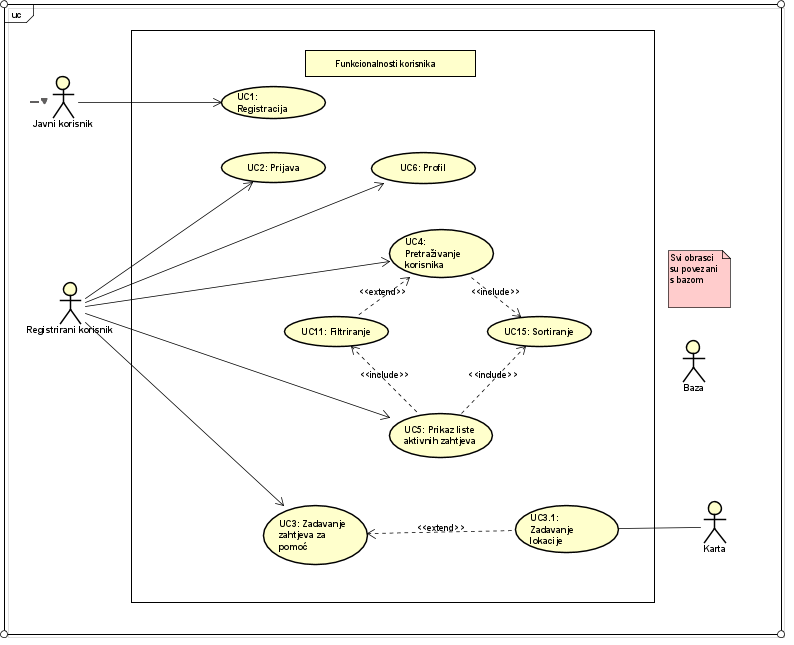
\includegraphics[scale=0.7]{slike/uc_funkcionalnosti_korisnika.png} %veličina slike u odnosu na originalnu datoteku i pozicija slike
	\centering
	\caption \newline Dijagram obrasca uporabe, funkcionalnosti korisnika
	\label{fig:promjene}
\end{figure}

%unos slike
\begin{figure}[H]
	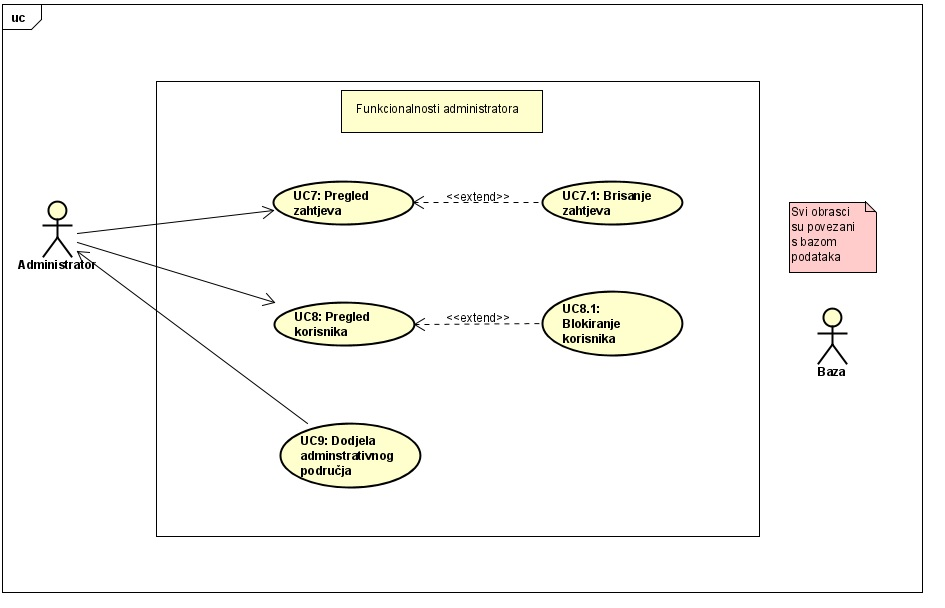
\includegraphics[scale=0.6]{slike/uc_funkcionalnosti_administratora.jpg} %veličina slike u odnosu na originalnu datoteku i pozicija slike
	\centering
	\caption \newline Dijagram obrasca uporabe, funkcionalnosti administratora
	\label{fig:promjene}
\end{figure}

%unos slike
\begin{figure}[H]
	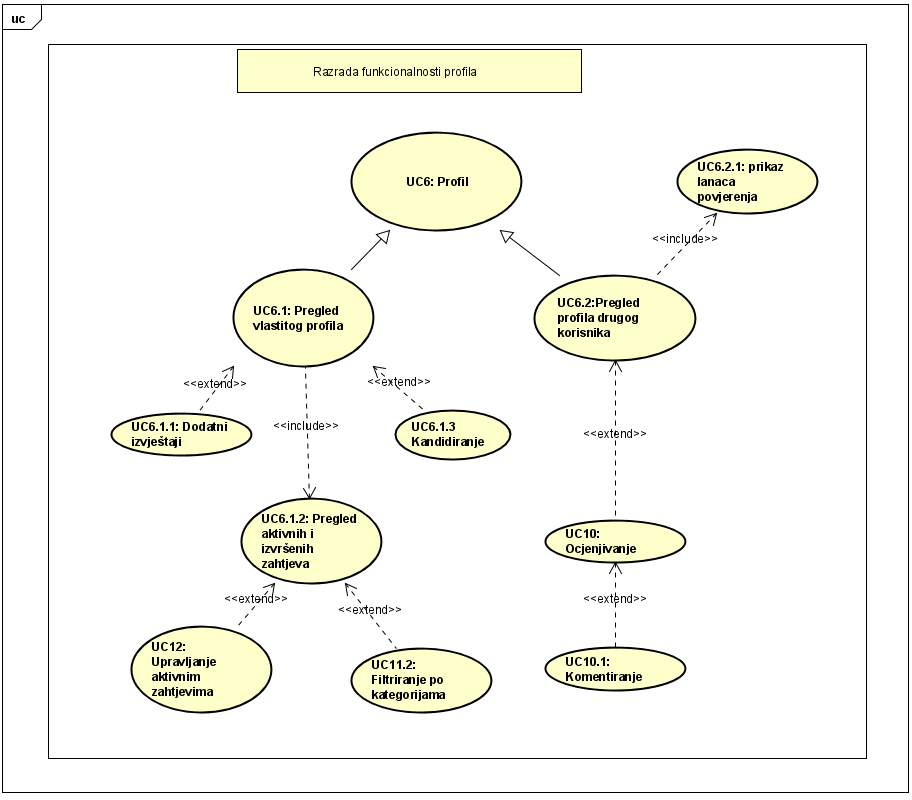
\includegraphics[scale=0.65]{slike/uc_profil.png} %veličina slike u odnosu na originalnu datoteku i pozicija slike
	\centering
	\caption \newline Dijagram obrasca uporabe, razrada funkcionalnosti profila
	\label{fig:promjene}
\end{figure}		

%unos slike
\begin{figure}[H]
	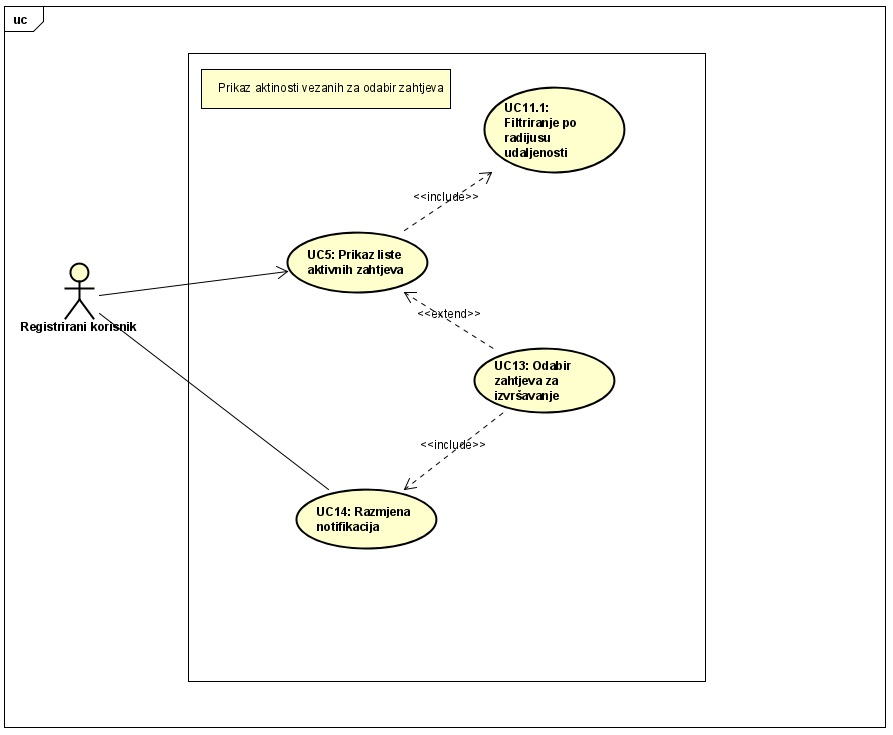
\includegraphics[scale=0.65]{slike/uc_odabir_zahtjeva.jpg} %veličina slike u odnosu na originalnu datoteku i pozicija slike
	\centering
	\caption \newline Dijagram obrasca uporabe, prikaz aktivnosti vezanih za upravljanje zahtjeva
	\label{fig:promjene}
\end{figure}

%unos slike
\begin{figure}[H]
	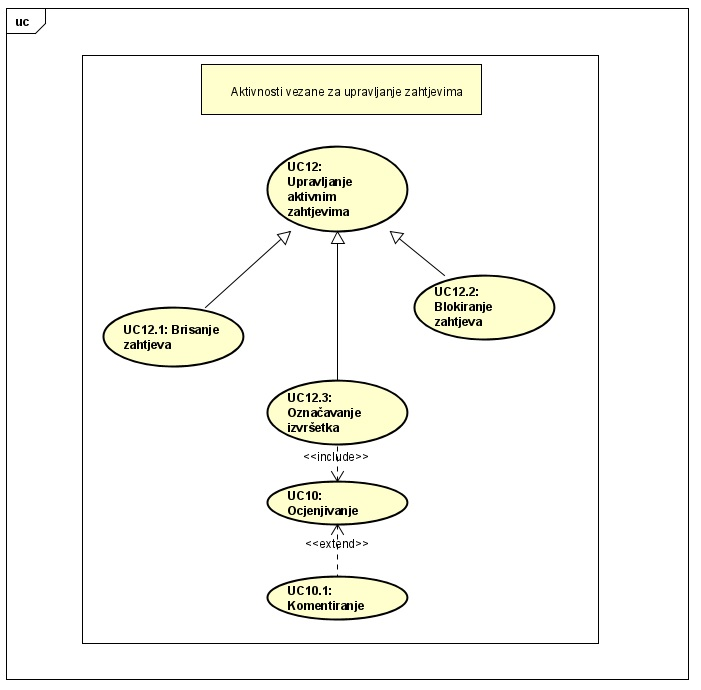
\includegraphics[scale=0.65]{slike/uc_upravljanje_zahtjevima.jpg} %veličina slike u odnosu na originalnu datoteku i pozicija slike
	\centering
	\caption \newline Dijagram obrasca uporabe, prikaz aktivnosti vezanih za odabir zahtjeva
	\label{fig:promjene}
\end{figure}

%unos slike
\begin{figure}[H]
	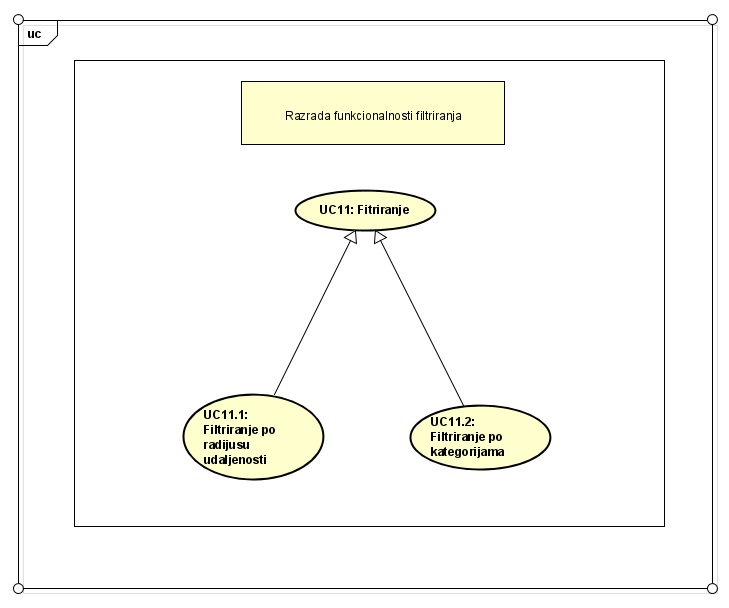
\includegraphics[scale=0.65]{slike/uc_filtriranje.jpg} %veličina slike u odnosu na originalnu datoteku i pozicija slike
	\centering
	\caption \newline Dijagram obrasca uporabe, razrada funkcionalnosti filtriranja
	\label{fig:promjene}
\end{figure}

\newpage

\subsection{Sekvencijski dijagrami}

\textbf{\textit{dio 1. revizije}}\\

\noindent {\textbf{Obrazac uporabe UC1 - Registracija }}
\newline\newline\textit {Korisnik šalje zahtjev za registracijom na sustav za primanje ili pružanje pomoći.
	Upisom registracijskih podataka,poslužitelj validira primljene podatke od strane
	korisnika.Ako je došlo do neuspješne validacije,poslužitelj o tome obavještava 
	korisnika ispisom poruke pogreške.Ukoliko su podaci ispravno validirani na
	strani poslužitelja,on prosljeđuje podatke prema bazi podataka.Baza podataka
	provjerava postajanje korisnika s identičnim ključnim podacim(email,lozinka).
	U slučaju postojanja korisnika s identičnim ključim podacima,baza podataka
	dojavljuje pogrešku sustavu,koji ona poruku proslijeđuje korisniku.Ako je provjera
	na strani baze uspješna,baza dojavljuje sustavu da je korisnik uspješno registriran,
	dok sustav korisniku ispisuje poruku uspješnosti.}\\


%unos slike
\begin{figure}[H]
	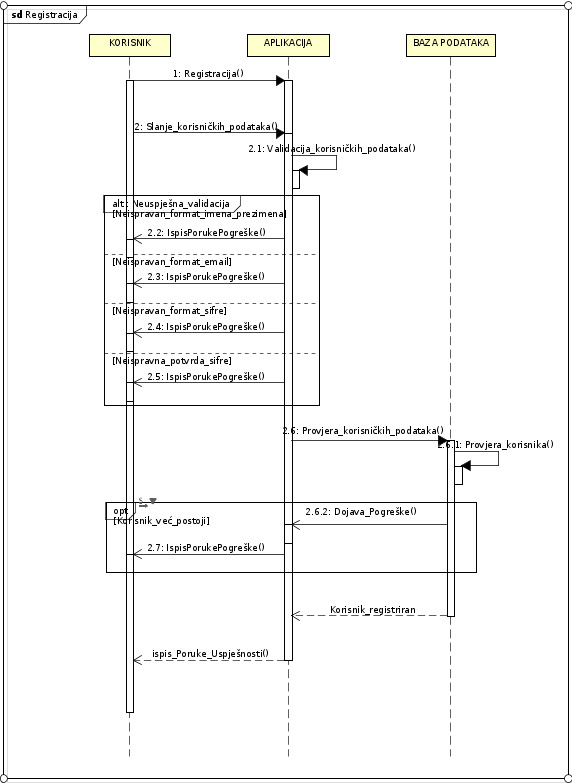
\includegraphics[scale=0.65]{slike/sekvencijski_dijagram_registracija.jpeg} %veličina slike u odnosu na originalnu datoteku i pozicija slike
	\centering
	\caption \newline Sekvencijski dijagram za UC1
	\label{fig:promjene}
\end{figure}

\newpage
\noindent {\textbf{Obrazac uporabe UC6 - Profil }}
\newline \newline {Korisnik prema poslužitelju šalje zahtjev za prikazom korisničkog profila.Poslužitelj
	iz baze dohvaća osnovne informacije o korisniku,komentare korisnika te dohvaća 
	visoko ocijenje korisnike korisnika koji je zatražio prikaz profila.Poslužitelj na temelju
	visoko ocijenjenih korisnika pretražuje eventualne njihove ocijene prema korisniku
	čiji se profil želi dohvatit i tako izgrađuje lanac povjerenja.Poslužitelj vraća
	osnovne informacije,komentare te lanac povjerenja korisniku koji je zatražio
	dohvat profila.}\\
\newline
%unos slike
\begin{figure}[H]
	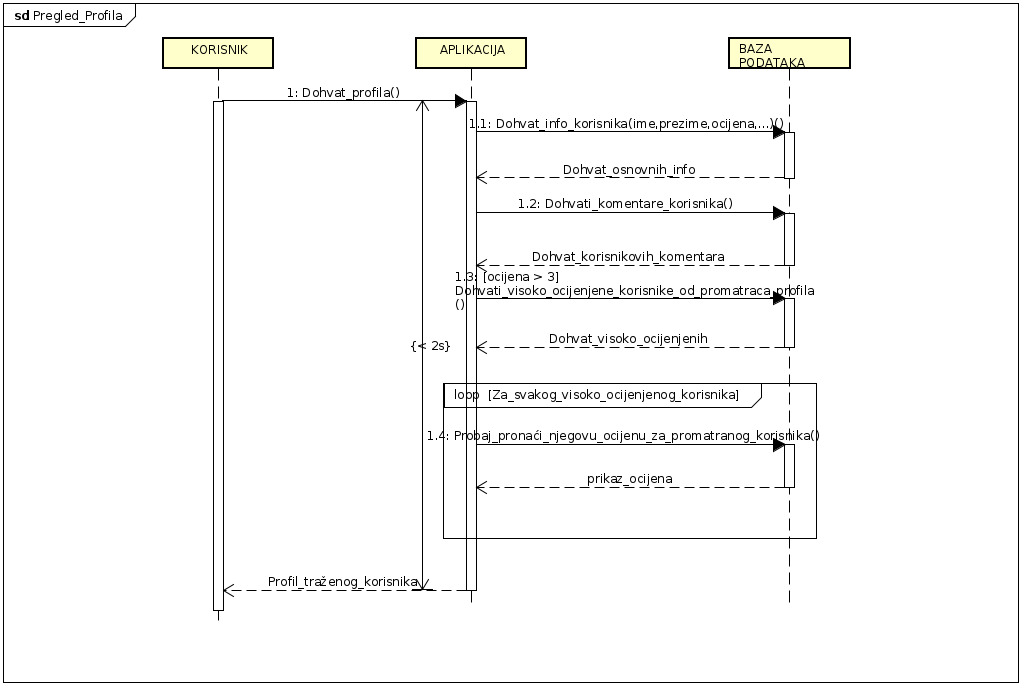
\includegraphics[scale=0.48]{slike/sekvencijski_dijagram_pregled_profila.jpeg} %veličina slike u odnosu na originalnu datoteku i pozicija slike
	\centering
	\caption \newline Sekvencijski dijagram za UC6
	\label{fig:promjene}
\end{figure}

\newpage
\noindent {\textbf{Obrazac uporabe UC3 - Zadavanje zahtjev za pomoć }}
\newline \newline  {Korisnik(autor) želi zadati novi zahtjev za pomoć.Unosi osnovne informacije koje su 
	potrebne za zahtjev te opcionalno unosi lokaciju ako ju smatra bitnom za zahtjev.
	Korisiku željenu lokaciju predaje poslužitlju u obliku geografaskih kordinata ili poslužitelj može
	automatski pomoću servisa za određivanje lokacije odrediti geografsku lokaciju uređaja s kojeg je zahtjev 
	zadan.Poslužitelj validira unesene informacije,ukoliko su unesene informacije neuspješno validiran poslužitelj
	dojavljuje pogrešku korisniku.Na kraju korisnik potvrđuje svoj zahtjev za pomoći.Poslužitelj prima zadani zahtjev 
	te prosljeđuje pohranu zahtjeva prema bazi podataka.Baza podataka potvrđuje uspješnu pohranu zahtjeva
	dok poslužitlej korisniku ispisuje poruku uspješnosti.}\\
%unos slike
\begin{figure}[H]
	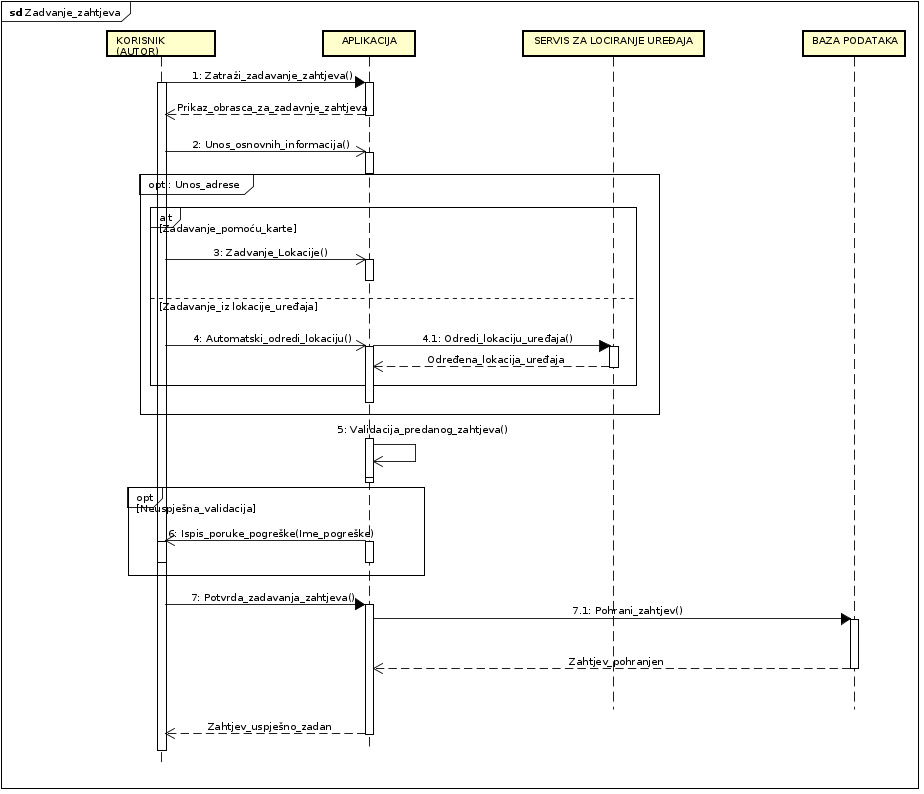
\includegraphics[scale=0.45]{slike/sekvencijski_dijagram_zadavanje_zahtjeva.jpeg} %veličina slike u odnosu na originalnu datoteku i pozicija slike
	\centering
	\caption \newline {Sekvencijski dijagram za UC3}
	\label{fig:promjene}
\end{figure}

\newpage
\noindent {\textbf{Obrazac uporabe UC13 - Odabir zahtjeva za pomoć }}
\newline \newline  {Korisnik šalje poslužitelju zahtjev za dohvat liste aktivnih zahtjeva.Poslužitelj
	dohvaća listu aktivnih zahtjeva iz baze podataka.Korisinik pregledava listu
	aktivnih zahtjeva uz mogućnost pregleda profila korisnika koji je zadao zahtjev.
	Korisnik odabire zahtjev s liste i prihvaća ga.Poslužitelj prima prihvaćanje zahtjeva
	te prosljeđuje promjenu u bazu podataka.Poslužitelj obavještava korisnika o uspješnoj pohrani 
	prihvaćanja zahtjeva.}\\
%unos slike
\begin{figure}[H]
	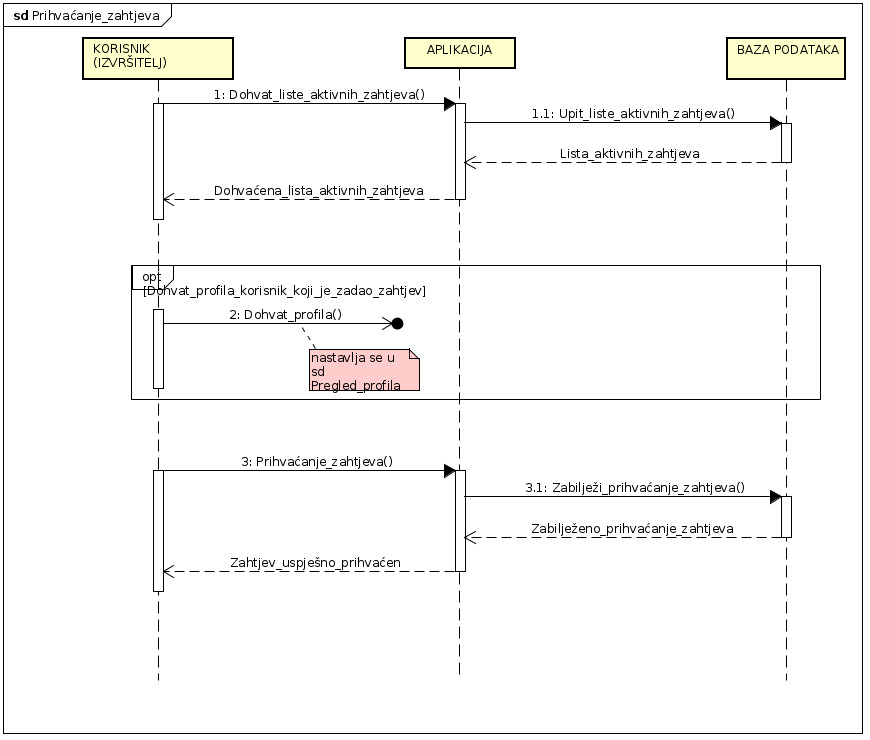
\includegraphics[scale=0.48]{slike/sekvencijski_dijagram_prihavcanje_zahtjeva.jpeg} %veličina slike u odnosu na originalnu datoteku i pozicija slike
	\centering
	\caption \newline Sekvencijski dijagram za UC13
	\label{fig:promjene}
\end{figure}

\newpage
\section{Ostali zahtjevi}


\
\begin{packed_item}
	\item Aplikaciju je moguće koristiti od strane više korisnika istovremeno
	\item Funkcionalnost sustava je neovisna o eventualnim greškama korisnika
	\item Baza podataka mora biti dobro konfigurirana i sigurna
	\item Korisnici pristupaju određenom geografskom području
	\item Implementacija je bazirana na objektno-orijentiranom jeziku
	\item Sustav mora omogućiti jednostavnu nadogradnju novih funkcionalnosti
	\item Aplikacija se koristi na standardnom hrvtaskom jeziku

\end{packed_item}
